%=======================================================================
%  GACI / TRA manuscript -- POLISHED Main results section (2026-06-30)
%  Drop-in replacement for the whole \section{Main results} (subsections,
%  tables, figures included). Terminology: "global aviation connectivity",
%  goods -> trade, each table/figure described, closing synthesis paragraph.
%  Figures used: GACI_implied_map.png, GACI_hetero_quartile.png,
%                GACI_continent_trend.png, GACI_shock_map.png  (all restyled).
%  NOTE: keep "trade = merchandise (goods), services excluded" once in Data.
%=======================================================================
\section{Main results}
%=======================================================================

We first ask whether global aviation connectivity raised trade openness, trade
volume, and GDP. Table~\ref{tab:main} reports, for each of our two measures of
global aviation connectivity, three lines side by side: the OLS association, the
first-stage relevance of the instrument, and the instrumented (2SLS) estimate.
Reading down each panel shows how isolating exogenous variation changes the
picture.

Panel A uses hub quality ($\ln\mathrm{GACI}_{cwm}$), our headline measure. The
instrument is a strong predictor of connectivity: it enters the first stage with
the expected positive sign ($0.032$, $p<0.01$), and the Kleibergen--Paap
statistic ($F=18.0$) sits comfortably above conventional weak-instrument
thresholds. In the second stage, a one-percent increase in hub quality raises
trade volume by about $2.3\%$ ($p<0.01$). This volume response decomposes into two
parts. Trade openness, the ratio of trade to GDP, rises by about $1.3\%$
($p<0.05$), and GDP rises by about $1.0\%$, although the GDP estimate is not
statistically significant. We treat trade openness as the headline result because
it isolates the pure trade effect net of economic scale: it measures whether
connectivity makes a country trade more relative to the size of its economy,
rather than simply enlarging the economy as a whole.

Panel B repeats the exercise with total connectivity ($\ln\mathrm{GACI}_{sum}$).
The qualitative picture is the same: volume and openness are positive and
significant, while the GDP effect is positive but imprecise. The two measures are
on different scales and cannot be compared coefficient for coefficient; what
carries over is the pattern of signs and significance, together with the exact
decomposition that holds in both panels.

\begin{table}[ht!]
\centering
\caption{Main results: OLS, first stage, and 2SLS, by connectivity measure (robust SE).}
\label{tab:main}
\begin{threeparttable}
\small
\begin{tabular}{lccc}
\toprule
 & Trade openness & Trade volume & GDP \\
 & $\ln(g/Y)$ & $\ln g$ & $\ln Y$ \\
\midrule
\multicolumn{4}{l}{\emph{Panel A. Hub quality, $\ln\mathrm{GACI}_{cwm}$ (headline)}}\\
First stage: instrument coef. & \multicolumn{3}{l}{0.032\sym{***}\ \ (0.007),\ \ KP $F=18.0$} \\
OLS & 0.157\sym{***} & 1.144\sym{***} & 0.987\sym{***} \\
2SLS & 1.302\sym{**} & 2.303\sym{***} & 1.001 \\
 & (0.662) & (0.776) & (0.680) \\
\addlinespace
\multicolumn{4}{l}{\emph{Panel B. Total connectivity, $\ln\mathrm{GACI}_{sum}$}}\\
First stage: instrument coef. & \multicolumn{3}{l}{0.064\sym{***}\ \ (0.020),\ \ KP $F=9.7$} \\
OLS & -0.027 & 0.237\sym{***} & 0.264\sym{***} \\
2SLS & 0.659\sym{*} & 1.166\sym{***} & 0.507 \\
 & (0.365) & (0.432) & (0.341) \\
\midrule
Country, Year FE & Yes & Yes & Yes \\
Observations & 4{,}643 & 4{,}643 & 4{,}643 \\
\bottomrule
\end{tabular}
\begin{tablenotes}\footnotesize
\item Robust (heteroskedasticity-consistent) SE in parentheses. Each panel
instruments its connectivity measure with the tourism-heritage instrument. The
first-stage row regresses the connectivity measure on the instrument (with
population and two-way FE); KP $F$ is the Kleibergen--Paap first-stage statistic.
Trade volume $=$ openness $+$ GDP by the identity $\ln g=\ln(g/Y)+\ln Y$.
\sym{*}~$p<0.10$, \sym{**}~$p<0.05$, \sym{***}~$p<0.01$.
\end{tablenotes}
\end{threeparttable}
\end{table}

To see where these gains fall, Figure~\ref{fig:impliedmap} maps each country's
implied trade gain, computed as its 2023 trade value times
$1-\exp(-\beta_{int}\,\Delta\ln\mathrm{GACI}_{cwm})$, the share of trade
attributable to that country's 1996--2023 rise in hub quality at the headline
openness elasticity $\beta_{int}=1.302$ (we sum these into a world total in
Section~\ref{sec:aggregate} below). The map shows the gains are highly
concentrated. China, Korea, the Gulf hubs (the United Arab Emirates and Saudi
Arabia), Turkey, and the fast-growing Southeast Asian economies show the largest
implied gains, having combined large connectivity increases with large trade
bases. A small set of advanced economies whose hub quality fell over the period,
chiefly Germany, Belgium, and Italy, register implied losses, while much of
Africa, Central Asia, and Latin America changes little.

\begin{figure}[t!]
\centering
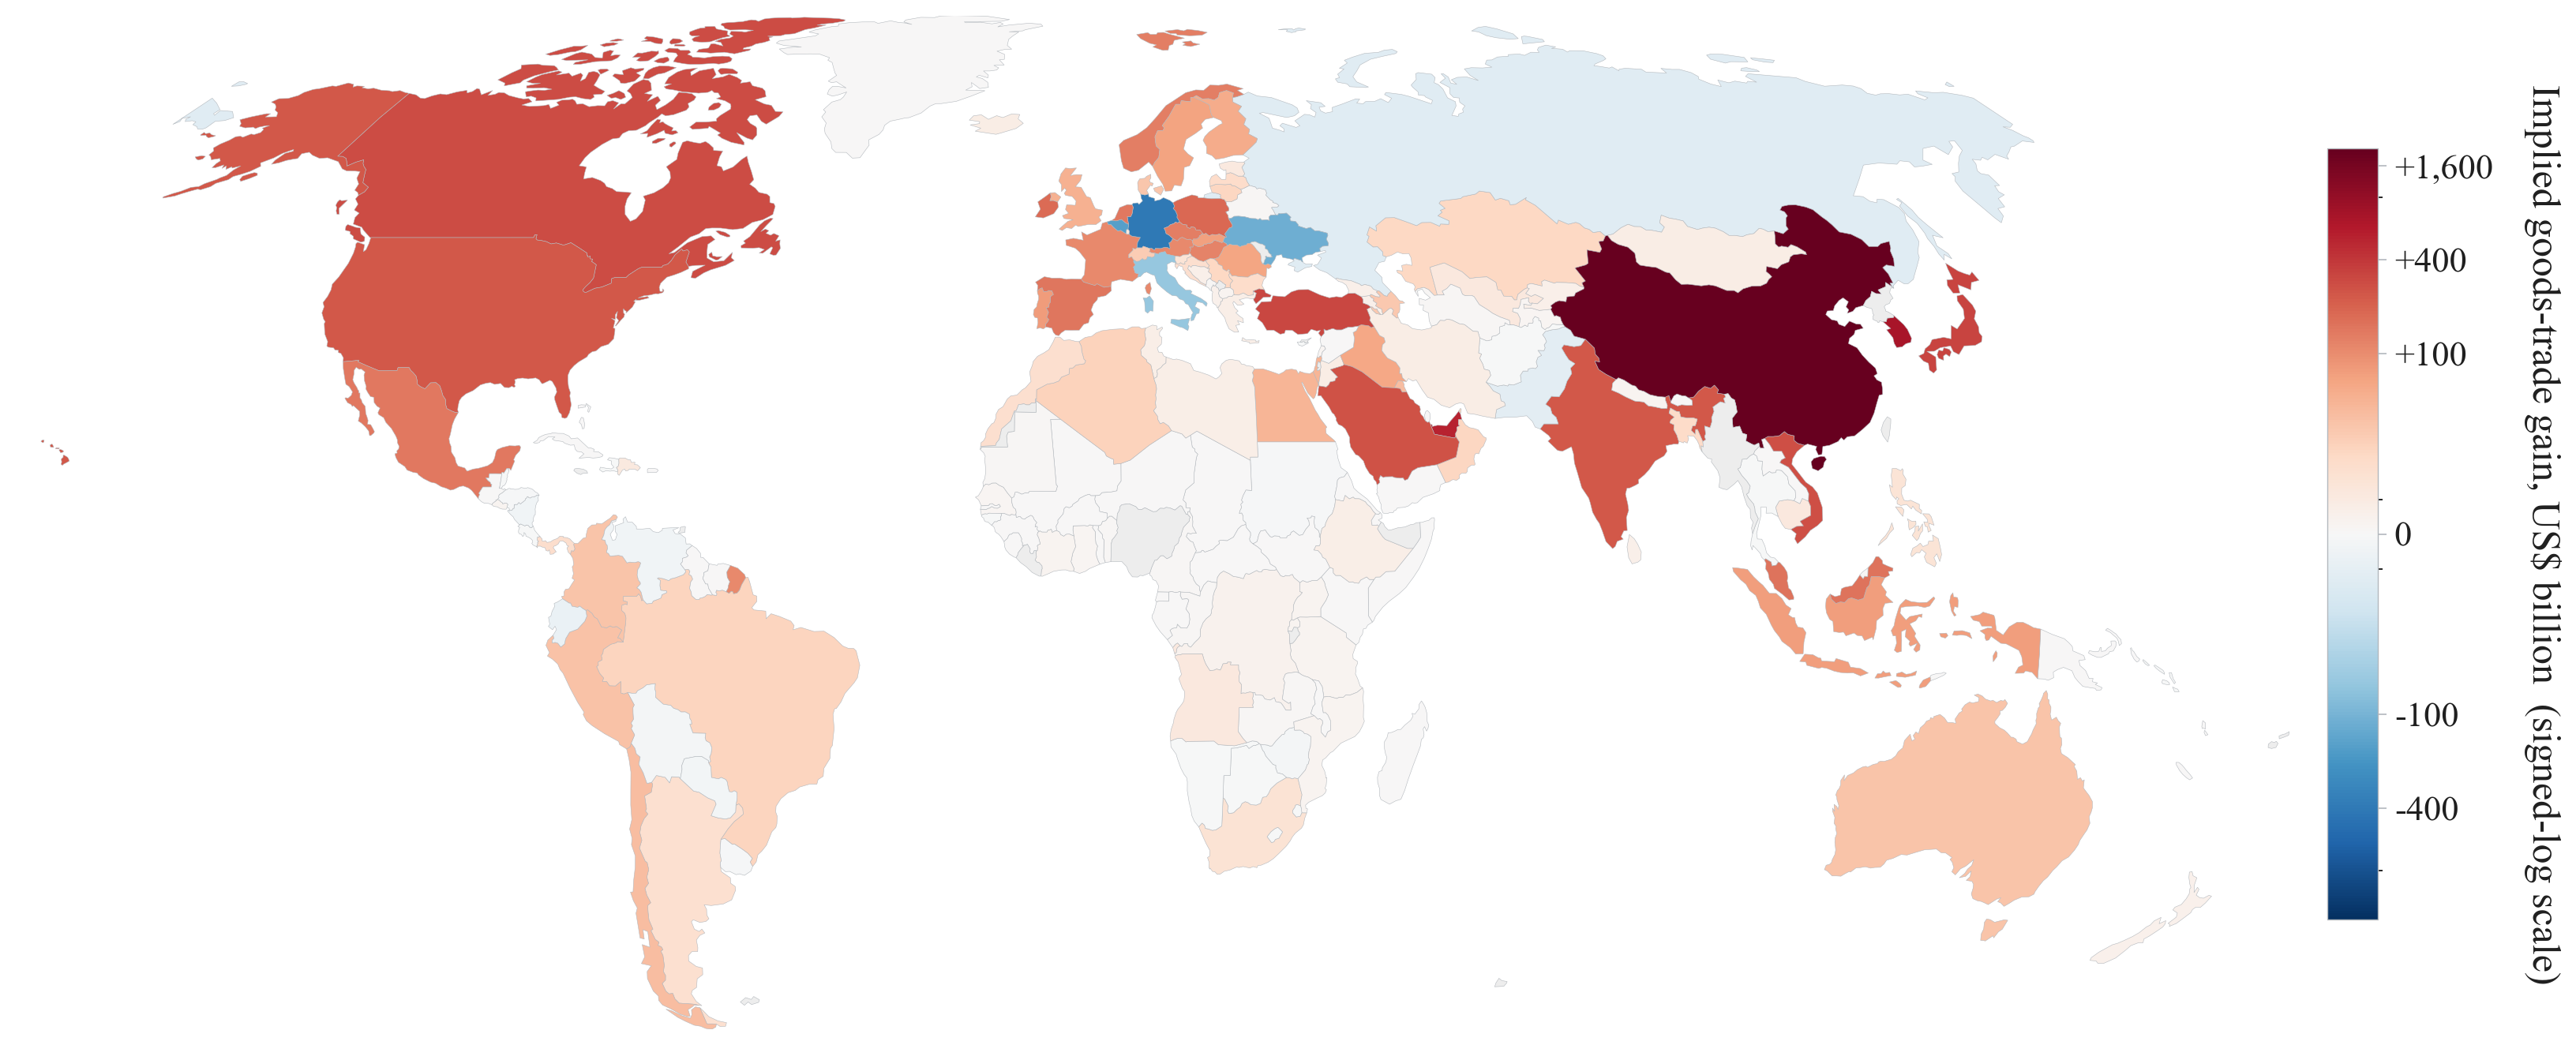
\includegraphics[width=\linewidth]{GACI_implied_map.png}
\caption{Implied trade gain from global aviation connectivity growth, 1996--2023
(intensity channel), $\beta_{int}=1.302$; signed-log colour scale.}
\label{fig:impliedmap}
\end{figure}

%=======================================================================
\subsection{Heterogeneity: who gains most?}
%=======================================================================

We next ask whether the average effect masks variation in who benefits, letting
the connectivity elasticity vary with three mean-centred baseline moderators:
income (log GDP per capita), global aviation connectivity ($\ln\mathrm{GACI}_{cwm}$),
and remoteness. Remoteness is each country's unweighted mean sea distance to all
other sample countries, from the CERDI sea-distance database, in logs; it is a
time-invariant, purely geographic measure (we use the unweighted mean because
GDP-weighting collapses to market proximity and inverts the ranking).
Table~\ref{tab:het} reports interaction-IV estimates: for each moderator,
``connectivity (at mean)'' is the effect for the average country and
``$\times$ moderator'' is how that effect shifts as the moderator rises, with both
the connectivity term and its interaction instrumented.

The interactions with baseline income and baseline connectivity are negative and
significant across all three outcomes: the payoff to connectivity is larger in
poorer and less-connected economies. Remoteness works the same way for openness
(more remote economies gain more in trade intensity) but is imprecise for volume
and GDP. Evaluated at the mean the effect remains positive and sizeable. The
interacted first stages are weaker (KP $F\approx5$--$9$), so we read the gradient
as a qualitative pattern and report every cell.

\begin{table}[ht!]
\centering
\caption{Heterogeneity: interaction IV (robust SE).}
\label{tab:het}
\begin{threeparttable}
\small
\begin{tabular}{lccc}
\toprule
Moderator (mean-centred): & Baseline income & Baseline conn. & Remoteness \\
\midrule
\multicolumn{4}{l}{\emph{Panel A. Trade openness $\ln(g/Y)$}}\\
Connectivity (at mean)   & 1.254\sym{*}  & 2.260\sym{*}  & 1.391\sym{**} \\
                         & (0.717)       & (1.161)       & (0.693) \\
$\times$ moderator       & $-0.243$\sym{**} & $-1.482$\sym{**} & $-1.241$\sym{*} \\
                         & (0.122)       & (0.622)       & (0.673) \\
\addlinespace
\multicolumn{4}{l}{\emph{Panel B. Trade volume $\ln g$}}\\
Connectivity (at mean)   & 1.959\sym{***} & 6.093\sym{***} & 2.394\sym{***} \\
                         & (0.732)       & (1.742)       & (0.825) \\
$\times$ moderator       & $-1.108$\sym{***} & $-6.060$\sym{***} & $-1.234$ \\
                         & (0.131)       & (1.046)       & (0.815) \\
\addlinespace
\multicolumn{4}{l}{\emph{Panel C. GDP $\ln Y$}}\\
Connectivity (at mean)   & 0.705         & 3.834\sym{***} & 1.003 \\
                         & (0.759)       & (1.133)       & (0.708) \\
$\times$ moderator       & $-0.865$\sym{***} & $-4.579$\sym{***} & 0.007 \\
                         & (0.119)       & (0.677)       & (0.755) \\
\midrule
First-stage KP $F$       & 8.07          & 4.96          & 9.21 \\
Country, Year FE         & Yes           & Yes           & Yes \\
Observations             & 4{,}121       & 4{,}121       & 4{,}635 \\
\bottomrule
\end{tabular}
\begin{tablenotes}\footnotesize
\item Each column is one moderator. Both $\ln\mathrm{GACI}_{cwm}$ and its
interaction with the (mean-centred) moderator are instrumented; country and year
FE; robust SE. Negative interactions on income and baseline connectivity
(significant across all three outcomes) mean the payoff is larger for poorer and
less-connected economies. KP $F$ is modest ($\approx5$--$9$), so the gradient is
qualitative. All cells reported, including the insignificant ones.
\sym{*}~$p<0.10$, \sym{**}~$p<0.05$, \sym{***}~$p<0.01$.
\end{tablenotes}
\end{threeparttable}
\end{table}

Figure~\ref{fig:hetquartile} makes this gradient concrete by plotting the implied
openness elasticity for each quartile of baseline income and baseline
connectivity. In both dimensions the elasticity falls monotonically from the
lowest to the highest quartile, from about $1.7$ to $0.8$ across income quartiles
and from about $2.7$ to $1.7$ across connectivity quartiles, though the confidence
intervals are wide, consistent with reading the pattern as qualitative.

\begin{figure}[ht!]
\centering
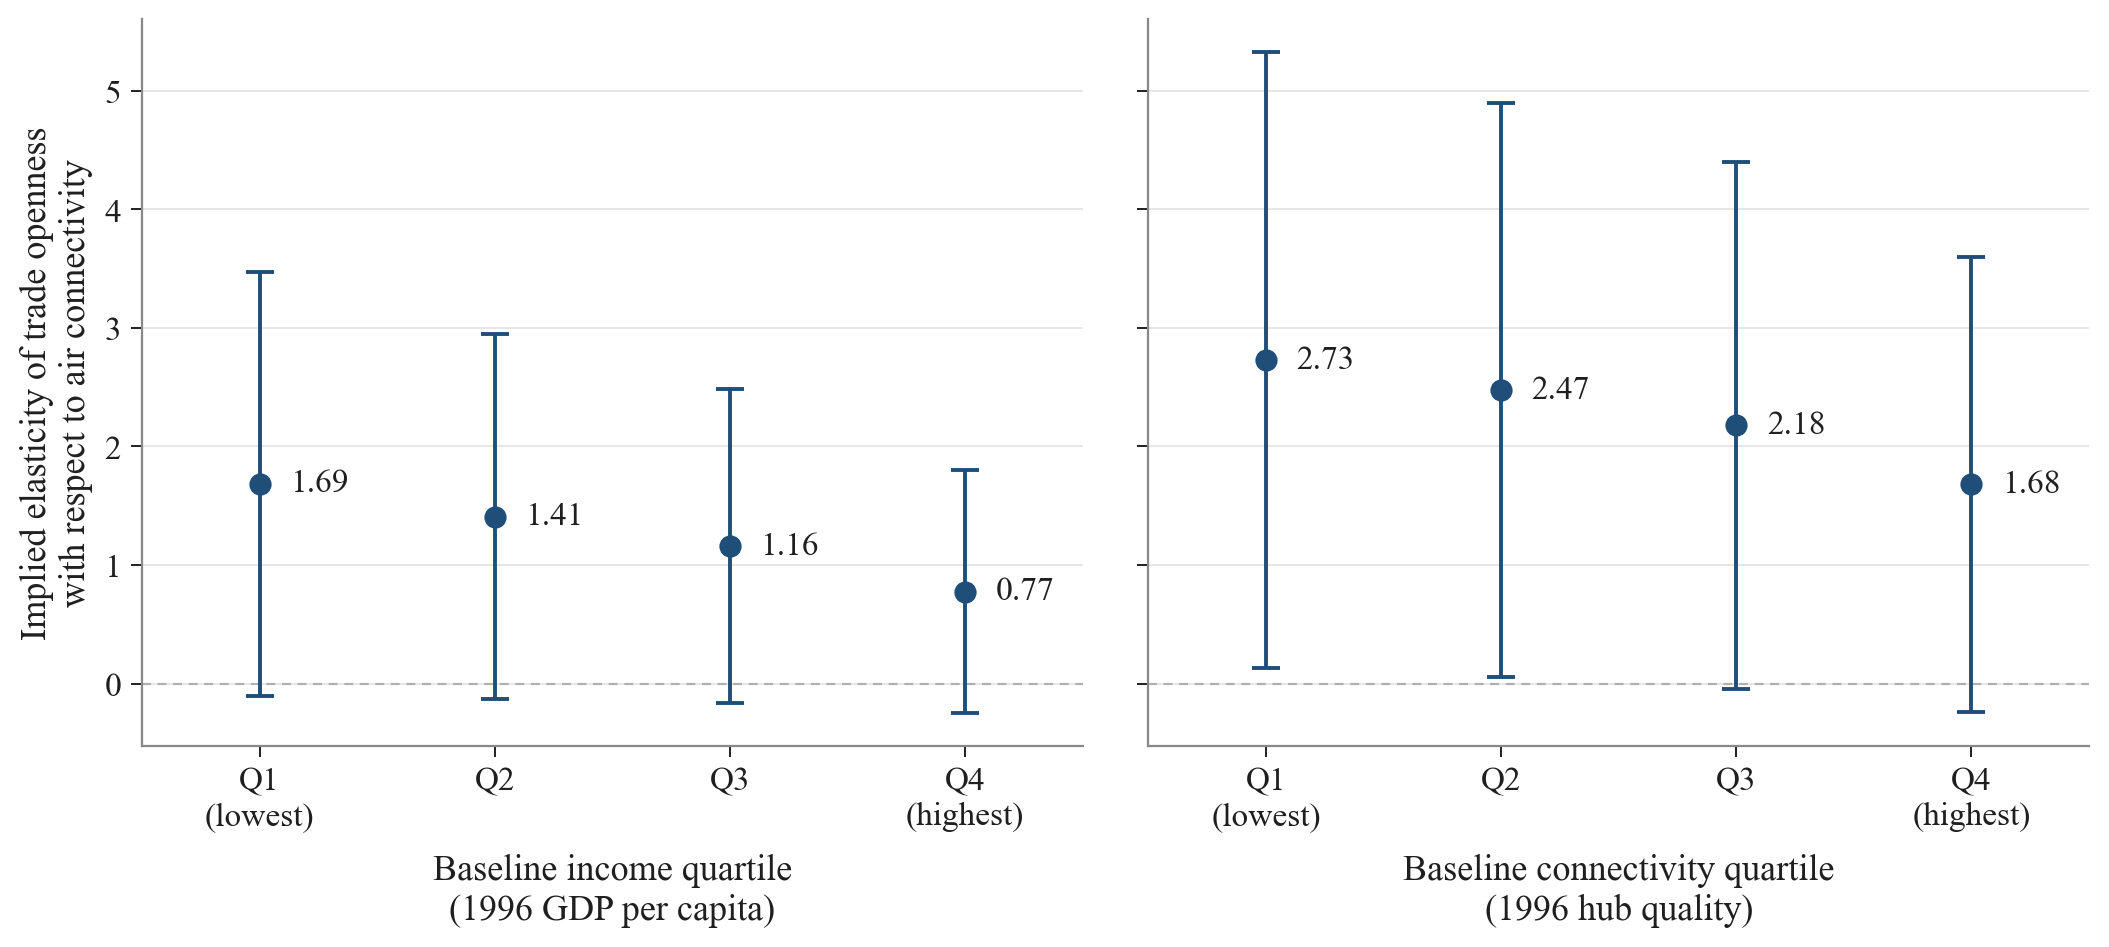
\includegraphics[width=0.95\linewidth]{GACI_hetero_quartile.png}
\caption{Implied elasticity of trade openness with respect to global aviation
connectivity, by baseline-income and baseline-connectivity quartile (Q1 = lowest;
95\% CIs).}
\label{fig:hetquartile}
\end{figure}

%=======================================================================
\subsection{Temporal heterogeneity}
\label{sec:temporal}
%=======================================================================
We also examine whether the effect has shifted over time by interacting global
aviation connectivity with a post-2010 indicator (Table~\ref{tab:temporal}). The
table reports the pre-2010 effect and how it changes after 2010 for each outcome.
The instrument is essentially irrelevant before 2010 (first-stage KP $F=0.29$) and
strong afterwards ($F=27.7$), so identification comes almost entirely from the
recent period. Consistent with this, under hub quality the post-2010 shift is
positive and significant for volume and GDP, so the impact is concentrated in the
post-2010 era of low-cost long-haul and Gulf and Asian hub expansion. Under total
connectivity the post-2010 first stage collapses and the sum interaction is not
identified; we report it with its large standard errors rather than omit it.

\begin{table}[ht!]
\centering
\caption{Temporal heterogeneity: interaction with post-2010 (robust SE).}
\label{tab:temporal}
\begin{threeparttable}
\small
\begin{tabular}{lccc}
\toprule
 & Trade openness & Trade volume & GDP \\
\midrule
\multicolumn{4}{l}{\emph{Treatment $=\ln\mathrm{GACI}_{cwm}$ (hub quality)}}\\
Connectivity (pre-2010) & 1.247   & 0.496   & $-0.751$ \\
                        & (0.771) & (0.877) & (0.983) \\
$\times$ post-2010      & 0.012   & 0.377\sym{***} & 0.366\sym{***} \\
                        & (0.076) & (0.088) & (0.091) \\
\addlinespace
\multicolumn{4}{l}{\emph{Treatment $=\ln\mathrm{GACI}_{sum}$ (total connectivity)}}\\
Connectivity (pre-2010) & 6.456   & 4.272   & $-2.184$ \\
                        & (22.75) & (13.65) & (10.26) \\
$\times$ post-2010      & $-0.334$ & $-0.179$ & 0.155 \\
                        & (1.205) & (0.724) & (0.542) \\
\midrule
Country, Year FE        & Yes & Yes & Yes \\
\bottomrule
\end{tabular}
\begin{tablenotes}\footnotesize
\item Country and year FE; robust SE. The instrument is essentially irrelevant
before 2010 (first-stage KP $F=0.29$) and strong afterwards ($F=27.7$), so
identification is concentrated in the post-2010 period. Under hub quality (cwm)
the effect on volume and GDP is significantly larger after 2010. Under total
connectivity (sum) the post-2010 first stage collapses, so the sum interaction is
not identified and is reported with its large SE rather than omitted.
\sym{*}~$p<0.10$, \sym{**}~$p<0.05$, \sym{***}~$p<0.01$.
\end{tablenotes}
\end{threeparttable}
\end{table}

%=======================================================================
\subsection{Aggregate contribution of connectivity growth, 1996--2023}
\label{sec:aggregate}
%=======================================================================
The elasticity in Table~\ref{tab:main} on its own says little about how much trade
is at stake. We therefore translate it into an aggregate magnitude. This serves
two purposes: it expresses the estimate in units that matter for policy (dollars
of trade and points of GDP), and it lets the contribution of two decades of global
aviation connectivity growth be compared against the size of the world economy.

The calculation is a partial-equilibrium counterfactual. For each country we ask
how much of its 2023 trade is attributable to that country's own 1996--2023 rise
in hub quality, holding everything else fixed. Applying the intensity (openness)
elasticity, the attributable share is
$1-\exp(-\beta\,\Delta\ln\mathrm{GACI}_{cwm,i})$ with $\beta=1.302$, so the
implied gain is
$\text{trade}_i\times\bigl(1-\exp(-\beta\,\Delta\ln\mathrm{GACI}_{cwm,i})\bigr)$;
summing across countries gives the world total.

On this basis, global aviation connectivity growth since 1996 is associated with
about \textbf{\$7.8 trillion} of 2023 trade, roughly \textbf{17\%} of 2023 world
trade (\$47 trillion) and \textbf{7.4\%} of 2023 world GDP, equivalently raising
world trade openness by about 7.4 percentage points of GDP. Figure~\ref{fig:continent}
traces the implied openness gain by continent over time and shows these gains
accrue most to the Middle East (Gulf hubs) and Asia (China), which pull away from
the rest after 2005.

\begin{figure}[ht!]
\centering
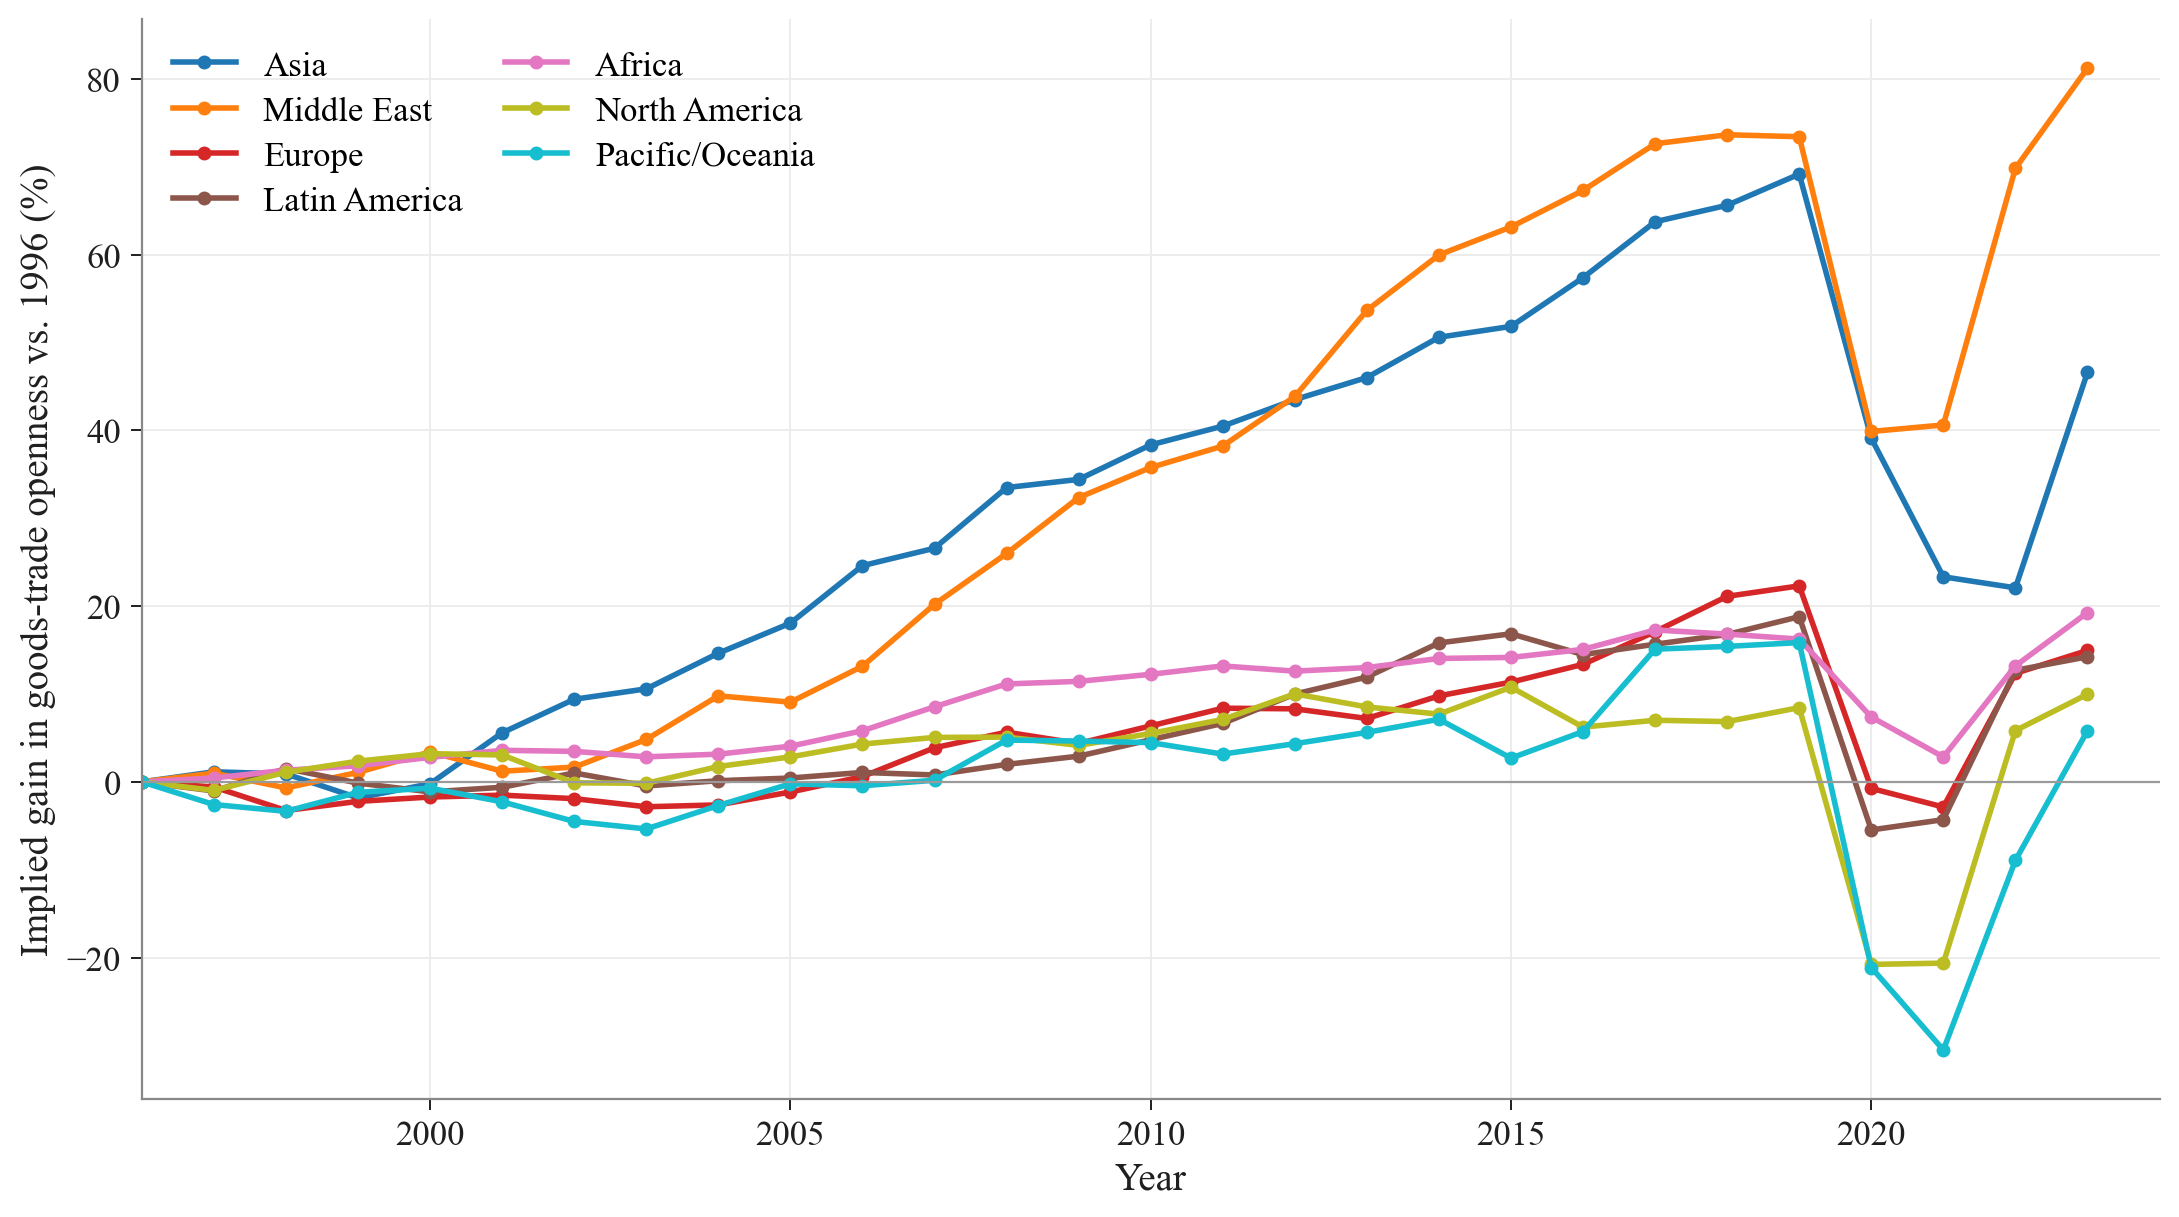
\includegraphics[width=0.9\linewidth]{GACI_continent_trend.png}
\caption{Implied gain in trade openness relative to 1996, by continent (intensity
channel, $\beta=1.302$).}
\label{fig:continent}
\end{figure}

%=======================================================================
\subsection{Connectivity-collapse shocks}
%=======================================================================
The same logic applies in reverse: if global aviation connectivity raises trade on
the way up, an abrupt collapse should subtract trade on the way down. For these
one-year shocks we measure the change in \emph{total} connectivity and apply the
corresponding sum intensity elasticity ($0.659$), because hub-quality means are
too volatile over a single year. In the COVID-19 collapse (2019 to 2020)
connectivity fell in 140 of 177 countries (median $\Delta\ln\mathrm{GACI}=-0.048$),
implying a trade disruption of about \$1.8 trillion, roughly 4.8\% of 2019 world
trade. Figure~\ref{fig:shock} maps this loss across countries and shows it is
concentrated in the major gateway hubs that had gained the most on the way up.

\begin{figure}[ht!]
\centering
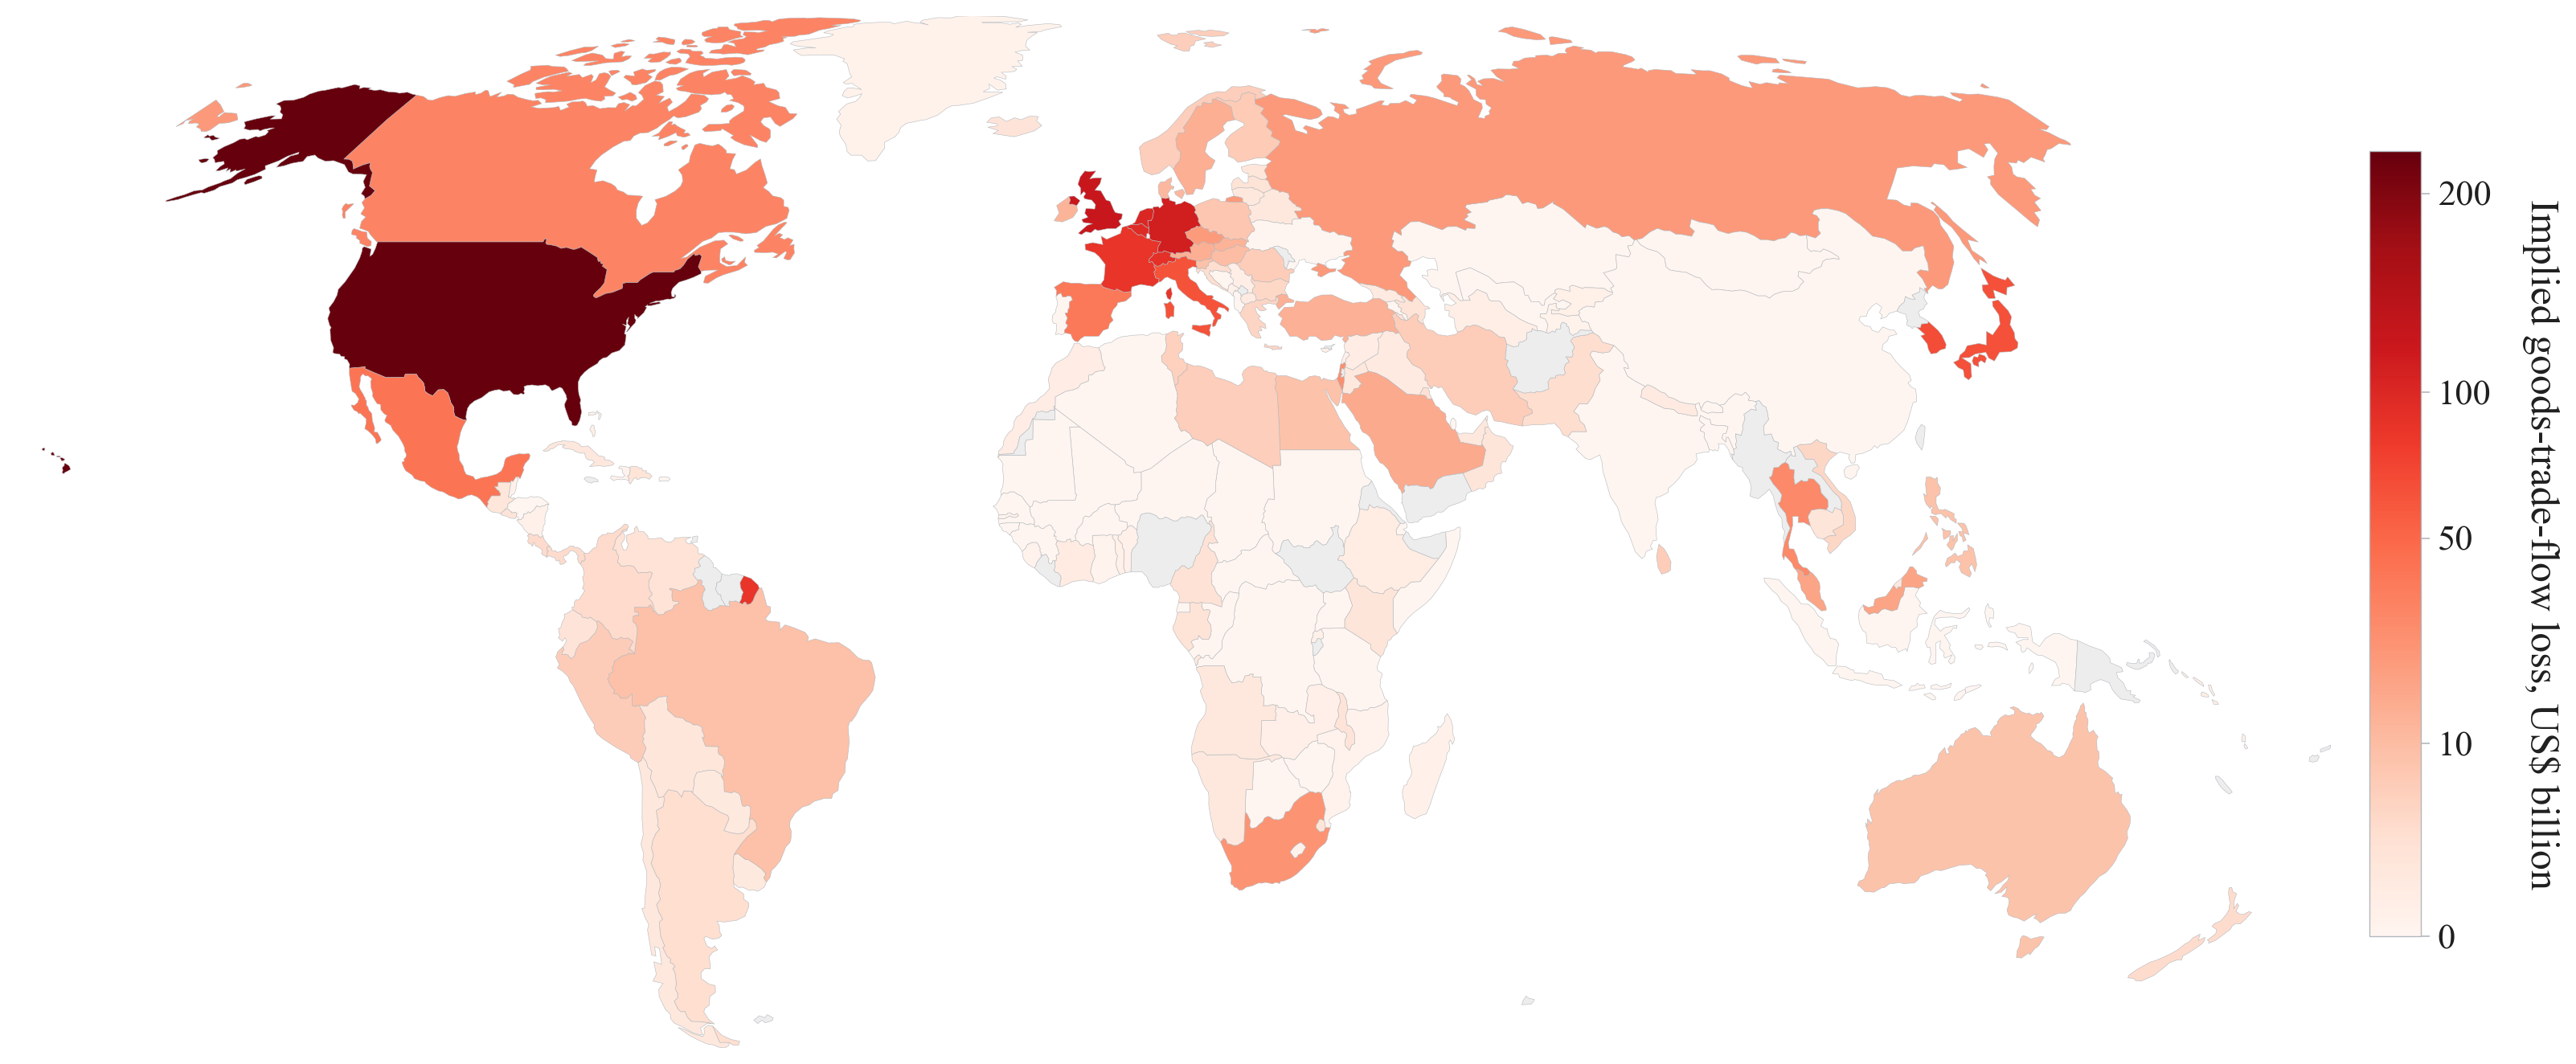
\includegraphics[width=0.9\linewidth]{GACI_shock_map.png}
\caption{COVID-19 (2019 to 2020): implied trade loss by country from the global
aviation connectivity collapse.}
\label{fig:shock}
\end{figure}

Taken together, these results carry four messages. First, global aviation
connectivity is a causal driver of trade integration, and it operates primarily on
the intensity margin: better-connected countries trade more relative to the size
of their economies, not merely because they are larger. Second, the returns are
unevenly shared and are largest for poorer, less-connected, and more remote
economies, so aviation acts as a convergence lever that substitutes for weak
surface and maritime access. Third, the relationship is concentrated in the
post-2010 era and is large in aggregate, accounting for about \$7.8 trillion of
2023 trade. Fourth, because connectivity builds trade on the way up, abrupt
collapses subtract it on the way down, as the COVID-19 episode shows. The policy
implication is direct: airport and route investment and air-service liberalisation
are concrete levers for trade integration, with the highest marginal returns in
peripheral economies.
